Una vez presentado el contexto, los objetivos, así como las herramientas empleadas, en este capítulo se detalla la mejora desarrollada sobre la herramienta Scratch4Robots. Primero presentamos el diseño global y después analizaremos en detalle que aportaciones se han realizado y como se han llevado a cabo.
\section{Diseño}
\label{sec:diseno}
Como diseño general de la herramienta, y la forma más sencilla de apreciar la sencillez con la que el usuario tiene que lidiar sería el siguiente esquema:
\begin{figure}[H]
    \centering
    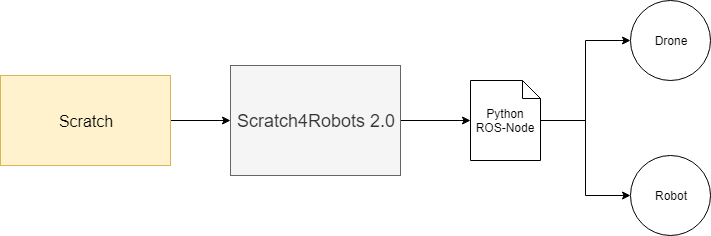
\includegraphics[scale=0.6]{img/s4r-diagram2.png}
  	\caption{Diseño de Scratch4Robots}
  	\label{fig:s4r}
\end{figure}

Para englobar todos los componentes ya definidos en un mismo contexto vamos a definir la arquitectura y diseño de la herramienta.
\begin{figure}[H]
    \centering
    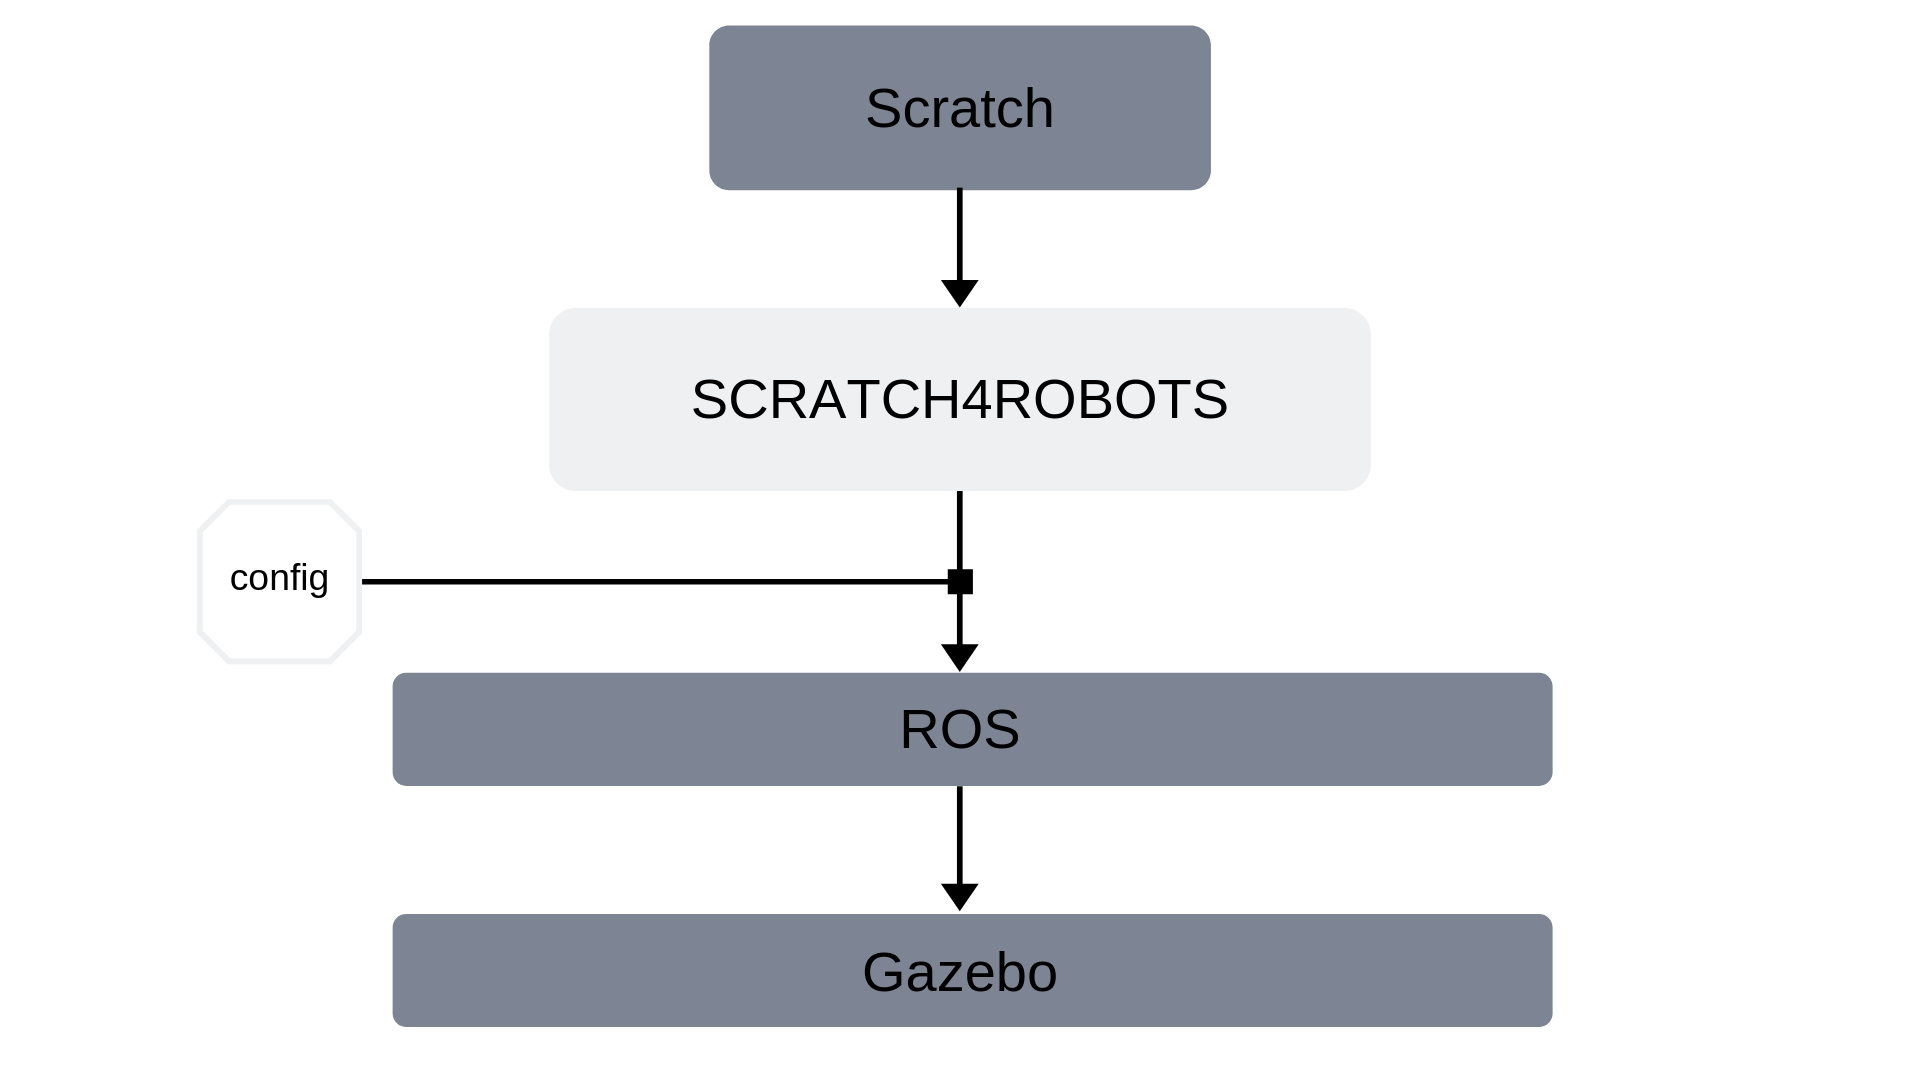
\includegraphics[scale=0.30]{img/diseno.jpg}
  	\caption{Diseño del contexto global de Scratch4Robots}
  	\label{fig:s4r}
\end{figure}
Partimos de un proyecto generado en el lenguaje de programación visual Scratch, al que se le ha agregado una serie de bloques robóticos, definidos e implementados por nosotros. Con estos nuevos bloques y los ya disponibles en Scratch se programará la lógica que queremos que siga nuestro robot.\\

Una vez tenemos nuestro proyecto, Scratch4Robots se encarga de la traducción de este proyecto a un nodo ROS, programado en Python, que con un único fichero de configuración en el que indicamos los tópicos que vamos a necesitar, se encuentra listo para su ejecución sobre un robot en un entorno simulado, por ejemplo Gazebo.\\

Esta traducción como hemos dicho devuelve un nodo ROS programado en Python, esto lo conseguimos introduciendo el código programado en scratch en una plantilla en la que se predefine toda la lógica necesaria para su ejecución.\\

Esta encapsulación del código generado en un nodo ROS la hemos conseguido través de la siguiente plantilla predefinida por nostros:

\begin{lstlisting}[language=python,firstnumber=1]
#!/usr/bin/env python
# -*- coding: utf-8 -*-n
import time
import config
import sys
import os
import yaml
import math
# Establece la subscripcion a topics ROS para drones
from drone import Drone 
# Establece la subscripcion a topics ROS para robots
from robot import Robot 

def execute(robot):
    try:
    # Desde codigo, insertamos la traduccion obtenida aqui 
    //
    except KeyboardInterrupt:
        raise
        
if __name__ == '__main__':
    if len(sys.argv) == 2:
        path = os.getcwd()
        open_path = path+'/'
        filename = sys.argv[1]
    else:
        sys.exit("ERROR: Example:python my_generated_script.py cfgfile.yml")
    # carga de configuraciones, topics ros a los que nos suscribimos, a traves de fichero yml.
    if os.path.isabs(filename):
        stream = open(filename, "r")
        cfg = config.load(filename)
    else:
        stream = open(open_path + filename, "r")
        cfg = config.load(open_path + filename)
        yml_file = yaml.load(stream)
        
    for section in yml_file:
    # En el yml de configuracion se define si se trata de robot o drone.
    if section == 'drone':
        # Si es drone se inicia la clase que hace la subscripcion a todos los topics ROS
        robot = Drone(cfg)
    	break
    elif section == 'robot':
    	# De forma analoga si se trata de un robot sobre ruedas
        robot = Robot(cfg)
    	break
    # Ejecutamos el codigo generado, ya con todas las subscriciones a ROS hechas
    execute(robot)

\end{lstlisting}


Esta plantilla abstrae de toda la dificultad tras la publicación y suscripción a tópicos ROS, y junto con el código traducido desde Scratch será el nodo final que el usuario ejecutará. Pero el proceso que hemos realizado para la completa integración con ROS no acaba aquí. Como se ve en la plantilla anterior, la suscripción a los topics se realiza a través de las librerías \textit{drone} y \textit{robot}. Esto se hace de cara a no sobrecargar el Nodo generado, con código que requiere de cierto nivel de entendimiento sobre la arquitectura ROS. Estos modulos python, que se facilita su uso mediante la instalación de los paquetes pip robot-scratch4robots y drone-scratch4robots, se encargan de la suscripción y publicación a los tópicos en los que nuestro robot simulado estrá conectado. Estas librerías han sido generados en su totalidad en esta versión de la herramienta, Scratch4Robots 2.0.\\

\begin{figure}[H]
    \centering
    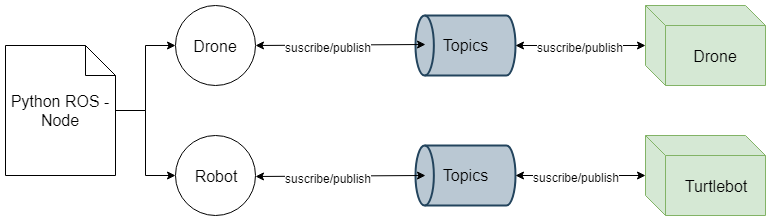
\includegraphics[scale=0.6]{img/s4r-diagrama-robot.png}
  	\caption{Esquema de funcionamiento del Nodo ROS en Python}
  	\label{fig:s4r-esquema}
\end{figure}

Entrando en más detalle de estas librerías, vamos a ver como realiza la suscripción y publicación en los tópicos desde una de ellas, con fragmentos de códigos obtenidos de la aplicación.\\

\begin{lstlisting}[language=python,firstnumber=1]
import config
import rospy

class Robot():
    def __init__(self, cfg):
        # inicia nodo ROS Robot
        self.__node = rospy.init_node("robot", anonymous=True)
        # hacemos la subscripcion a los topics ROS
        topic = cfg.getProperty("robot.Pose3D.Topic")
        self.__pose3d_client = ListenerPose3d(topic)
        topic = cfg.getProperty("robot.Motors.Topic")
        self.__motors_client =  PublisherMotors(topic)
\end{lstlisting}

Describiendo el fragmento de código anterior y como se aprecia en el esquema de más arriba, nuestro nodo ROS en Python, a través del objeto Python \textit{Robot}, hace la carga de propiedades del cfg que se le pasa como argumento. Estas propiedades como hemos comentado anteriormente serán los tópicos a los que se conectará nuestro nodo. Se realizará la suscripción a cada tópico de manera individual. En este caso y observando el código,  usamos el objeto \textit{ListenerPose3d}, para conectarnos al tópico de el que obtendremos la información publicada por el sensor de odometría del robot, del mismo modo se hace con \textit{PublisherMotors} para el uso de los motores del robot.\\

En el siguiente extracto de código se aprecia simplificado el detalle de una de las clases que realizan la suscripción, y de las obtenemos información del robot a través de mensajes ROS, publicados en un tópico.

\begin{lstlisting}[language=python,firstnumber=1]
# modulo python oficial ros
import rospy
# mensajes de comunicacion ROS para la lectura de odometria
from nav_msgs.msg import Odometry
class ListenerPose3d:
    def __init__(self, topic):
    	# Objeto Pose3d() contiene los datos devueltos por el sensor
        self.data = Pose3d() 
        # Al suscribirnos como argumento se introduce el topico,
        # el tipo de mensaje ROS que se lee del topico
# y una funcion de callback en la que recogemos las lecturas del topico
        self.sub = rospy.Subscriber(self.topic, Odometry, self.__callback)

    def __callback (self, odom):
        pose = odometry2Pose3D(odom)
        self.lock.acquire()
        self.data = pose
        self.lock.release()
        
    # metodo a traves del cual obtendremos la pose 3d    
    def getPose3d(self):
        self.lock.acquire()
        pose = self.data
        self.lock.release()
        return pose
\end{lstlisting}

Este mismo procedimiento hay que seguirlo para cada uno de los posibles tópicos ROS que necesite nuestra aplicación, por ejemplo, uno para dar velocidad a los distintos motores, otro para el sensor láser, cámaras incrustadas en el robot etcétera.

Con todo esto se puede apreciar la complejidad de la que evadimos al usuario, siendo para él, un simple ejecutable o nodo, completamente operativo, generado a través de nuestra aplicación. Una vez lanzado el nodo habremos sido capaces de aplicar una lógica programada en Scratch sobre un robot en un entorno simulado. 


\section{Desarrollo de bloques}
\label{sec:desarrollo-de-bloques}

Una de las aportaciones de este trabajo a la herramienta ha sido la refactorización de bloques ya existentes y la agregación de nuevos bloques funcionales.
En la programación visual entendemos por bloque a cada componente visual que contiene una lógica específica, con la agrupación de bloques podemos conseguir un flujo de programación complejo. En primer lugar vamos a describir como agregar estos nuevos bloques a Scratch, siguiendo con su definición e implementación.

\subsection{Extensión de Scratch}

Scratch facilita el uso de bloques personalizados mediante extensiones externas, estas  extensiones externas a la aplicación se definen mediante el uso de ficheros JSON, aunque por convención, en Scratch tendrán extensión .s2e. Este tipo de ficheros se creó para la comunicación mediante HTTP de bloques con aplicaciones auxiliares, por ejemplo algún tipo de hardware. Nosotros no vamos a utilizar esta funcionalidad, únicamente nos ayudamos de este documento .s2e para definir nuestra extensión y pueda ser usada desde el IDE offline de scratch.\\

En este documento se define un objeto JSON, el cual será la definición de la extensión, en el que se incluye el nombre de la extensión, un puerto usado para la comunicación de componentes externos en caso de ser necesario y una lista de bloques de Scratch. \\

A continuación se define un ejemplo de una extensión para Scratch. 
\begin{lstlisting}[language=json,firstnumber=1]
{ 
  "extensionName": "Extension Example",
  "extensionPort": 12345,
  "blockSpecs": [
    [" ", "beep", "playBeep"],
	[" ", "set beep volume to %n", "setVolume", 5],
	["r", "beep volume", "volume"],
  ]
}
\end{lstlisting}

El campo ``blockSpecs'' describe los bloques de extensión que aparecerán en el apartado ``Más bloques'' en la aplicación de Scratch.
En en este caso, hay tres bloques:
\begin{itemize}
\item Un bloque de comandos que reproduce un pitido.
\item Un bloque de comando que
establece el volumen del pitido.
\item Un bloque que devuelve un valor, que informa del volumen de un pitido.
\end{itemize}

Cada bloque se describe mediante una matriz con los siguientes campos:
\begin{itemize}
\item \textbf{Tipo de bloque}:

\begin{itemize}
\item ' ' - bloque de comandos
\item 'w' - bloque de comandos que esperan
\item 'r' - bloque que retorna un valor
\item 'b' - bloque que retorna un booleano 
\end{itemize}
\item \textbf{Formato de bloque}:

El formato de bloque es una cadena que describe las etiquetas y ranuras de parámetros que aparecen en el bloque.
Las ranuras de parámetros están indicadas por una palabra que comienza con '\%' y puede ser una de:
\begin{itemize}
\item \%n -  parámetro de número 
\item \%s - parámetro de cadena 
\item \%b - parámetro booleano
\end{itemize}
\item \textbf{Operación o nombre de variable remota}:

El campo de operación en una especificación de bloque se usa de dos maneras. Para bloques de comandos, se envía a la aplicación auxiliar, junto con cualquier valor de parámetro, para invocar una operación. O para retornar bloques, es el nombre de una variable de sensor. Los valores de la variable del sensor se guardan en un diccionario.
La ejecución de un bloque simplemente devuelve el valor reportado más recientemente para esa variable de sensor.
\item \textbf{Parámetros predeterminados}:

Se pueden añadir cero o más valores de parámetros predeterminados

\item \textbf{Menús desplegables}:

Los bloques que definimos pueden hacer uso de parámetros de menú, los cuales definiremos de dos formas:
\begin{itemize}
\item \%m.menuName - parámetro de menú (no editable), proporciona un sencillo espacio para los parámetros del menú desplegable.
\item \%d.menuName - parámetro de número editable con menú, proporciona una ranura de parámetro numérico con un menú auxiliar.
\end{itemize}
\end{itemize}

Con todo esto podemos entender la definición de alguno de nuestros bloques como podemos en el siguiente extracto de código, en el que se ve la definición de algunos de nuestros bloques.
\begin{nobreak} 
\begin{lstlisting}[language=json,firstnumber=1]
{
  "extensionName": "Scratch4Robots",
  "extensionPort": 12345, 
  "blockSpecs": [
    ["", "stop robot-drone", "stop"],         
    ["", "move robot %m.robotDirections speed %n", "robot/move/speed", "forward", 1],
    ["r", "color detection %m.color", "camera/all","red"],
    ["r", "frontal laser distance", "laser/frontal"],
  ],
  "menus": {
    "robotDirections": ["forward", "back"],         
    "color": ["red", "blue"]
  }
}

\end{lstlisting}
\end{nobreak} 

\subsection{Bloques genéricos}
Antes de comenzar con los bloques propios a nuestra extensión vamos a necesitar una serie de bloques genéricos que nos ayuden a realizar lógica básica de programación como pueden ser operadores matemáticos, operadores lógicos y sentencias básicas de programación. Scratch ya nos ofrece estos bloques por definición, por lo que no hará falta agregarlos a nuestra extensión específica, solamente nos encargaremos de su posterior traducción a código Python.\\

A continuación mostramos todos los bloques genéricos de los que podemos hacer uso desde la herramienta Scratch4Robots, ya que hemos implementado su traducción a Python.

\begin{itemize}
\item \textbf{Bloques de operadores matemáticos}:

Bloques fundamentales de cara a realizar una lógica posterior con los datos obtenidos desde los sensores de nuestros robots, estos bloques son una de las mejoras ofrecidas por este trabajo.
\begin{figure}[H]
    	\centering
    	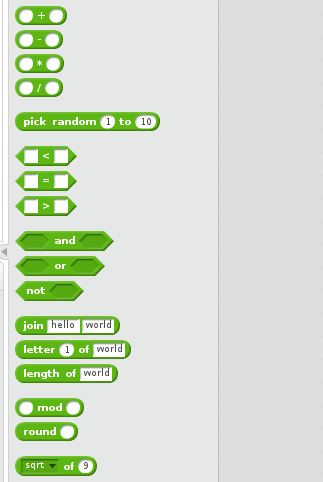
\includegraphics[scale=0.60]{img/bloques-mat.png}
     	\caption{Bloques matemáticos y lógicos}
  	\label{fig:mat}
\end{figure}

	\begin{itemize}

    \item \textbf{sqrt of ()}: Realiza la operación raíz cuadrada de un número dado
    \item \textbf{sin of ()}: Realiza la operación seno de un número dado
    \item \textbf{cos of ()}: Realiza la operación coseno de un número dado
    \item \textbf{tan of ()}: Realiza la operación tangente de un número dado
    \item \textbf{asin of ()}: Realiza la operación arcoseno de un número dado
    \item \textbf{acos of ()}: Realiza la operación arcocoseno de un número dado
    \item \textbf{atan of()}: Realiza la operación arcotangente de un número dado
    \item \textbf{log of ()}: Realiza la operación logaritmo de un número dado
    \item \textbf{ln of ()}: Realiza la operación logaritmo neperiano de un número dado
    \item \textbf{abs of ()}: Devuelve el valor absoluto de un número
    \item \textbf{mod of ()}: Devuelve el módulo de un número dado
    \end{itemize}

\item \textbf{Bloques de operadores lógicos}:
Permiten construir expresiones lógicas, se obtiene como resultado booleanos.
\begin{itemize}

 \item \textbf{And}: Operador de conjunción.
 \item \textbf{Or}: Operador de disyunción.
 \item \textbf{NOT}: Operador de negación.
 \item \textbf{Mayor que y Menor que}: Operadores de comparación numérica.
\end{itemize}

\item \textbf{Bloques de control}:

Estructuras de control básicas de programación.

\begin{figure}[H]
    	\centering
    	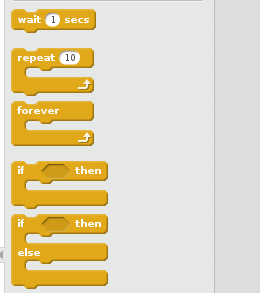
\includegraphics[scale=0.60]{img/bloques-control.png}
     	\caption{Bloques de control}
  	\label{fig:control}
\end{figure}
\begin{itemize}
\item \textbf{Wait () secs}: Pausa la ejecución el tiempo especificado, equivalente a la sentencia \textit{time.sleep()} de Python.
\item \textbf{Forever}: Bucle infinito, equivalente a \textit{while(True)} en lenguaje Python.
\item \textbf{If () then}: Comprueba la condición para que si la condición es verdadera, los bloques dentro de ella se ejecuten.
\item \textbf{If () Then, Else}: Comprueba la condición para que si la condición es verdadera, los bloques dentro de la primera condición se activen y si la condición es falsa, los bloques dentro de la segunda condición se activarán.
\item \textbf{Repeat ()}: Un ciclo que repite la cantidad de veces especificada, sería la equivalencia al bucle \textit{for} en Python.
\end{itemize}
\item \textbf{Otros}
\begin{itemize}

\item \textbf{say ()}: Imprime lo que le añadas como argumento, equivalente a \textit{print}.
\item \textbf{Set () to ()}: Utilizado para dar valor a una variable en concreto.
\end{itemize}

\item \textbf{Bloques de listas}:

Esta serie de bloques desarrollados en esta versión han sido de gran ayuda a la hora de la refactorización y creación de otros bloques de mayor complejidad.

\begin{figure}[H]
     	\centering
     	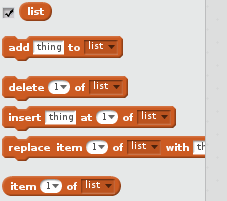
\includegraphics[scale=0.60]{img/bloques-listas.png}
     	\caption{Bloques de listas}
  	\label{fig:listas}
\end{figure}

\begin{itemize}
\item \textbf{Insert () at () of ()}: Inserta elemento en la posición seleccionada de la lista indicada.
\item \textbf{Item () of ()}: Devuelve el elemento almacenado en la posición indicada de la lista.
\item \textbf{Add () to ()}: Inserta en la lista un elemento.
\item \textbf{Delete () of ()}: Elimina el elemento en una posición determinada de la lista.
\end{itemize}
\end{itemize}

\subsection{Bloques para drones}
Estos bloques ya pertenecen a la extensión creada para la herramienta.
En este trabajo se ha realizado una refactorización completa de todos los bloques referentes a drones y la agregación de nuevos bloques. 

Cabe destacar de estos bloques que una vez traducidos al nodo final, que se consigue implementar el funcionamiento de drones bajo comunicación ROS, ésto es algo elaborado completamente en este trabajo.\\

Para ello nos apoyamos en MAVROS\footnote{\url{http://wiki.ros.org/mavros}}, puente oficial entre nodos ROS y Mavlink\footnote{\url{https://github.com/mavlink}}, el protocolo de comunicación estándar para drones.

\begin{itemize}
\item \textbf{Bloques perceptivos}:
Nos permiten obtener información de sensores incorporados en el drone.
	\begin{itemize}
	\item \textbf{Get pose3D}: Obtiene el valor de la posición 3D del robot.
		\begin{figure}[H]
     		\centering
     		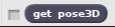
\includegraphics[scale=1.2]{img/block-pose.png}
     		\caption{bloque que retorna la posición del robot}
  		\label{fig:listas}
		\end{figure}
Simplificando la totalidad del código, la función Python en la que quedaría traducida sería \textit{getPose3d}, como se muestra:\\

\begin{lstlisting}[language=python,firstnumber=1]
class Drone():
    def __init__:
        client__pose3d = suscribePose3d(topic)
    def getPose3d(self):
        return client__pose3d.getPose3d
\end{lstlisting}
	\item \textbf{Color detection}: Nuevo componente añadido en esta versión, que haciendo uso de una cámara en el robot, detecta objetos de un determinado color, introducido como argumento, devolviendo una lista que contendrá las posiciones en los ejes x e y, además del tamaño del objeto, en la imagen capturada por la cámara.\\
	\begin{figure}[H]
     		\centering
     		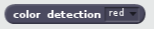
\includegraphics[scale=1.2]{img/block-color.png}
     		\caption{bloque que detecta objetos de un determinado color}
  		\label{fig:listas}
  				\end{figure}
  				
 Usando la biblioteca OpenCV de Python y con técnicas de análisis computacional de imágenes, de una simple imagen somos capaces de obtener su posición en la imagen y su tamaño:\\
 
 \begin{lstlisting}[language=python,firstnumber=1]
    def detect_object(self, color):
        # define the lower and upper boundaries of the basic colors
        color_range = __get_color_range(color)
        # get image type from camera ROS client
        image = self.__camera_client.getImage()
        # apply color filters to the image
        filtered_image = cv2.inRange(image.data, color_range[0], color_range[1])
        rgb = cv2.cvtColor(image.data, cv2.COLOR_BGR2RGB)
        # Apply threshold to the masked image
        ret,thresh = cv2.threshold(filtered_image,127,255,0)
        im,contours,hierarchy = cv2.findContours(thresh,cv2.RETR_TREE,cv2.CHAIN_APPROX_SIMPLE)
        # Find the index of the largest contour
        for c in contours:
            if c.any != 0:
                areas = [cv2.contourArea(c) for c in contours]
                max_index = np.argmax(areas)
                cnt=contours[max_index]
                if max(areas) > 0.0:
                    x,y,w,h = cv2.boundingRect(cnt)
                    x_position = (w/2)+x
                    y_position = (h/2)+y
                    size = w*h
        return size, x_position, y_position
\end{lstlisting}


	\end{itemize}
\item \textbf{Bloques de movimiento}
	\begin{itemize}
	\item \textbf{Stop robot-drone}: Pone a su valor inicial todas las velocidades del robot.\\
	\begin{figure}[H]
     		\centering
     		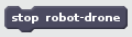
\includegraphics[scale=1.2]{img/block-stop.png}
     		\caption{bloque stop-robot}
  		\label{fig:listas}
  				\end{figure}
Con el código que se ejecutará tras su traducción:\\

 \begin{lstlisting}[language=python,firstnumber=1]
    def stop_robot(self):
        self.client__vel.sendVelocities(0,0,0,0,0,0)
        time.sleep(1)

\end{lstlisting}

	\item \textbf{Drone take off}: Hace que el drone despegue.\\
	\begin{figure}[H]
     		\centering
     		
\includegraphics[scale=1.2]{img/block-takeoff.png}
     		\caption{bloque que realiza el despegue del drone}
  		\label{fig:listas}
  				\end{figure}
  				
Mediante el armado del drone y el envío de una velocidad ascendente conseguimos su despegue:\\

 \begin{lstlisting}[language=python,firstnumber=1]
    def takeoff(self):
        self.client__extra.arming()
        self.client__vel.sendVelocities(0,0,2,0,0,0)
        time.sleep(1)
        self.client__vel.sendVelocities(0,0,0,0,0,0)
\end{lstlisting}

	\item \textbf{Drone land}: Realiza un aterrizaje controlado del drone.\\
	\begin{figure}[H]
     		\centering
     		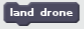
\includegraphics[scale=1.2]{img/block-land.png}
     		\caption{bloque que realiza el aterrizaje del drone}
  		\label{fig:listas}
  				\end{figure}
Para realizar el aterrizaje del drone a través de ROS, tiene su propio tópico al cual se le envía una llamada con argumentos cero, como se puede observar:\\

 \begin{lstlisting}[language=python,firstnumber=1]
    def land(self):
        self.lock.acquire()
        self.land_client.call(0,0,0,0,0)
        self.lock.release()
\end{lstlisting}
	

	\item \textbf{Move drone}: Bloque que tras la refactorización admite una lista con las velocidades del drone en los diferentes ejes (velocidad en el eje x, velocidad en el eje z, velocidad yaw), pare realizar giros se debe combinar la velocidad en el eje x con la velocidad de rotación en yaw.\\
	\begin{figure}[H]
     		\centering
     		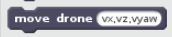
\includegraphics[scale=1.2]{img/block-move-drone.png}
     		\caption{bloque que realiza el despegue del drone}
  		\label{fig:listas}
  	\end{figure}
  	
Lo que se traduce a python con la siguiente función:\\
  	
\begin{lstlisting}[language=python,firstnumber=1]
 def move_vector(self, velocities):
    # cliente que realiza la suscripcion al topico que envia velocidades
    pose = self.client__pose3d.getPose3d()
    yaw = pose.yaw
    vx = velocities[0]
    vz = velocities[1]
    az = velocities[2]
    vxt = vx*math.cos(yaw)
    # cliente que realiza la suscripcion al topico que envia velocidades
    self.client__vel.sendVelocities(vxt,0,vz,0,0,az)
\end{lstlisting}
	
	Para clarificar la creación del cliente, y ver donde se realiza la comunicación ROS realmente se adjunta un estracto de código en el que se simplifica el cliente que publica el tópico en el que se van a enviar las velocidades al drone.\\
	
\begin{lstlisting}[language=python,firstnumber=1]
class publisher_motors:
    # simplificando el codigo del cliente
    def __init__(self, topic):
        self.pub = rospy.Publisher(topic, TwistStamped, queue_size=1)

    def sendVelocities(vx,vy,vz,ax,ay,az):
        tw = vel2twisted(vx,vy,vz,ax,ay,az)
        self.pub.publish(tw)
\end{lstlisting}
	
	\end{itemize}
\end{itemize}



\subsection{Bloques para robots con ruedas}
\begin{itemize}
\item \textbf{Bloques perceptivos}
	\begin{itemize}
	\item \textbf{Pose3D} :Obtiene el valor de la posición 3D del robot.
		\begin{figure}[H]
     		\centering
     		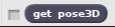
\includegraphics[scale=1.2]{img/block-pose.png}
     		\caption{bloque pose del robot}
  		\label{fig:listas}
  	\end{figure}
Se traduce de forma equivalente a su homólogo para drones, la única diferencia es el tópico desde el que recibe la información.\\
 
	\item \textbf{Color detection}: Bloque homólogo al del drone, dado un color nos devuelve su posición en la imagen, y su tamaño.
		\begin{figure}[H]
     		\centering
     		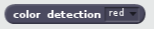
\includegraphics[scale=1.2]{img/block-color.png}
     		\caption{bloque que detecta colores en una imagen}
  		\label{fig:listas}
  	\end{figure}
Se trata del mismo bloque perceptivo ya definido para drones.\\

\item \textbf{Frontal distance}: Obtiene la medida promedio de los datos del láser frontal. 
		\begin{figure}[H]
     		\centering
     		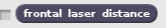
\includegraphics[scale=1.2]{img/block-laser.png}
     		\caption{bloque que devuelve datos de un laser}
  		\label{fig:listas}
  	\end{figure}
Se traduce al siguiente método Python:\\

\begin{lstlisting}[language=python,firstnumber=1]
def get_laser_distance(self):
        # get laser values from ROS client
        laser = self.__laser_client.getLaserData()
        l = [x for x in laser.values if str(x) != 'nan' and x < 10]
        try:
            avg = sum(l) / len(l)
        except ZeroDivisionError:
            avg = 0
        return avg
\end{lstlisting}

	\end{itemize}
\item \textbf{Bloques de movimiento}
	\begin{itemize}

	\item \textbf{robot move ()}: Admite como parámetro una lista con las velocidades en el eje x e y.
		\begin{figure}[H]
     		\centering
     		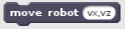
\includegraphics[scale=1.2]{img/block-move-robot.png}
     		\caption{bloque de movimiento para robots}
  		\label{fig:listas}
  	\end{figure}
  	
Con su traducción:\\

\begin{lstlisting}[language=python,firstnumber=1]
    def move_vector(self, velocities):
        vx = float(velocities[0])
        vz = float(velocities[1])
        print "velocities:",vx,vz
        self.__reset()
        self.__vel.vx = vx
        self.__vel.vz = vz
        if vz>0:
            self.turn("left",vz)
        if vz<0:
            self.turn("right",vz)
        self.__publish(self.__vel)
\end{lstlisting}

	\item \textbf{robot turn ()}: Permite la rotación sobre el propio eje del robot.
	\begin{figure}[H]
     		\centering
     		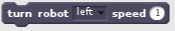
\includegraphics[scale=1.2]{img/block-turn.png}
     		\caption{bloque que realiza el giro del robot}
  		\label{fig:listas}
  	\end{figure}
  	
Con su traducción Python:\\

\begin{lstlisting}[language=python,firstnumber=1]
    def turn(self, direction, vel):
        self.__vel.az = vel
        # set different direction
        if direction == "right":
            self.__vel.az = -self.__vel.az
        # publish movement
        self.__publish(self.__vel)
\end{lstlisting}
	\end{itemize}
\end{itemize}

Con esto se definen los bloques pertenecientes a nuestra extensión, de la forma en que Scratch los muestra y la traducción de cada uno de ellos llevada, de una forma simplificada. Se aprecia que se trata de robots sofisticados, con cierta complejidad. La cual hacemos transparente para el usuario, simplificando toda la lógica que existe tras cada robot, en simples e intuitivos bloques gráficos.

\section{Traducción de bloques}
El último paso será definir la estrategia que vamos a seguir para realizar la traducción de los bloques creados anteriormente, al nodo ROS final, programado en Python.

Vamos a estudiar más a fondo como trabaja la biblioteca Kurt y cómo nos ha ayudado en la traducción de bloques.\\

Kurt es una biblioteca de Python que permite la manipulación compleja de proyectos Scratch (archivos .sb o .sb2) a través de simples comandos de Python. Incluye un decompilador, que permite que un proyecto se cargue en un conjunto de objetos de Python, y un compilador que permite el empaquetamiento de un conjunto de scripts de imágenes / texto en proyectos scratch.\\

En este proyecto se ha utilizado una versión\footnote{\url{https://pypi.org/project/jderobot-kurt/}} mejorada de esta biblioteca, con ciertas adaptaciones para el tratamiento de extensiones externas como la nuestra. Kurt define los bloques usados por Scratch como objetos JSON, en esta nueva versión se agrega un fichero con la configuración de nuestros bloques como objetos JSON. De esta forma se agrega la capacidad de obtener la información de los bloques de nuestra extensión.\\

La clase principal de kurt almacena el contenido de un archivo de proyecto Scratch.
Los contenidos incluyen variables globales y listas, el escenario y los sprites, cada uno con sus propios scripts, sonidos, variables y listas.\\

Una vez obtenido el contenido de un proyecto Scratch en un objeto Python, con el siguiente fragmento de código somos capaces de obtener el String representativo de cada bloque.\\

\begin{lstlisting}[language=python,firstnumber=1]
# load the scratch project
p = kurt.Project.load(open_path + sys.argv[1])

# show the blocks included
for scriptable in p.sprites + [p.stage]:
	for script in scriptable.scripts:
		# exclude definition scripts
		if "define" not in script.blocks[0].stringify():
			s = script
print("Stringify:")
sentences = []
for b in s.blocks:
	print(b.stringify())
\end{lstlisting}

Una vez tenemos la lista de los Strings equivalentes a los bloques del proyecto Scratch, hay que realizar una tarea de transformación de estas a código Python.\\

En este trabajo se modifica de forma notable la forma en la que se realizaba de forma inicial esta traducción, agregando una gran cantidad de bloques soportados y añadiendo un grado de recursividad que permite la traducción de bloques anidados.\\

En la traducción nos apoyamos de unos diccionarios Python en los que mapeamos el string equivalente al bloque Scratch con el equivalente Python que queremos sustituir, esto nos lleva al último punto de nuestro desarrollo. Para ciertos bloques de Scratch existe una traducción directa a un comando Python como ya hemos visto antes. Mientras que para los bloques robóticos definidos por nuestra extensión debemos de crear un método específico que contenga toda la lógica a implementar como hemos visto anteriormente en la descripción de nuestros bloques.\\

En este trabajo hemos refactorizado la totalidad de la lógica tras los bloques robóticos, dándole una mayor coherencia a todos ellos. Además de crear lógica completamente nueva para ciertos bloques agregados en esta versión. Cabe destacar el bloque referente a la detección de objetos de un cierto color.\\

Además de la traducción, Scratch4Robots encapsula este código Python en un nodo ROS, que contiene todo lo necesario para su posterior ejecución, con el único requisito de un fichero de configuración en el que especificaremos los tópicos que va a necesitar nuestro nodo. Cerrando de esta forma el ciclo de trabajo de la herramienta.\\





